\chapter{Background and Related Work}
\label{chap:stateOfTheArt}

\begin{chapterintro}
The following section discusses the actual approaches in the area of packet parsing, classification and data processing. 
These operations are tightly bound and they need to be solved as effectively as possible because 
they are the keys for the effective and fast data processing in high-speed computer networks.
The section also introduces available abstract descriptions of packet processing devices. 
\end{chapterintro}

\section{Problem Statement}
% Tady se opet bude opakovat definice tri zakladnich operaci
% 1) Parsovani
% 2) Klasifikace
% 3) Obecne zpracovani (stavove zpracovani)
%
% Podrobny popis v odstavcich jednotlivych skupin
%
% Dale bude dobre najit vysokourovnove popisy pro popis sitoveho HW. Jsou v podstate dva Gorilla, Xilinx SDN, P4. 
% To je dulezite, protoze to budeme pouzivat jako vstup a melo by se dat namapovat na nas HW.

In this section, we define three fundamental network operation groups, which are the core components of each network device. 
From the packet processing point of view, we can define three groups of operations:
\begin{enumerate}
	\item Data Extraction/Packet Parsing
	\item Classification
	\item Data Processing (we will talk about stateful processing)
\end{enumerate}

The first group, Data Extraction, must precede all other groups like classification, routing, filtering of incoming traffic, and so on. 
Each incoming packet must pass through some sort of parsing block to understand what is transferred inside the network packet. 
The examined data is then used in next stages which are related to classification or 
data processing. Therefore, the parsing is the first action which is performed on incoming network packet and it has to be carefully 
designed to support the expected packet rate of network interface. 
For example, the maximal packet rate for 10\,Gbps Ethernet with minimal packet length (64 bytes) equals to 1,488,096 packets per second. 
The network device should be able to process it without any problems. 
It can be otherwise a bottleneck of the system. A simple parsing example can be extraction of the IP address, TCP ports, or MAC address.

Classification is tightly bound to packet parsing and it is typically the second operation in the packet processing chain. 
The packet classification means the categorization of incoming packets into classes. 
The extracted protocol fields form an identifier, which is used for searching of processing rule. 
Rule is typically stored in a database of rules. 
This database is searched with packet identifier for the best matching record. 
Matched rule contains the identifier of the action, which is to be performed on the packet. 
For example, the network switch extracts the destination MAC address which is used for searching of an output port. 

The last stage of the packet processing is the Data Processing block. This block is typically designed to perform some operations like data changing, 
advanced filtering based on pattern matching, and so on. 
This stage of packet processing typically accepts read rule from the classification and 
parsing stage to perform a predefined operation which can be set from a software tool or it can be hard-wired in the networking device. 
The graphical representation of 
the packet processing concept is shown in Fig.~\ref{fig:packetProc}. 
In some cases, we can have more classification and action stages to implement more complex operations
like reaction to modified set of header fields (e.g., filtering of traffic behind NAT) and so forth.

\begin{figure}[ht]
	\centering
	\includegraphics[width=\textwidth]{chapters/pic/frame_data_process}
	\caption{Base packet processing pipeline.}
	\label{fig:packetProc}
\end{figure}


\section{Fundamental Network Operations}
% Napsat, ze ted budeme mluvit o state-of-the-art jednotlivych skupin s ohledem i na pripadnou praci v oblasti popisu
% pomoci high-level urovne. Hlavne se tu bude mluvit o resenich, ktere jsou nejvetsim prinosem v jednotlivych oblastech

The following text describes the current state-of-the-art of briefly introduced groups from the packet processing point of view. 
We introduce the cutting edge solutions because they are the starting point for our further research.

\subsection{Parsing}
\label{sec:parsing}
% State of the art pro parsovani

Network communication is divided into layers. Each layer has some task which is required for success delivery of network data.
The typical structure of a packet consists of a stack of protocol headers and payloads. 
Each protocol adds its own protocol header which is understandable 
by the same network layer on the other device. This is shown in Fig.~\ref{fig:osi}. The main task of the packet parsing is the extraction of 
protocols headers, which are added during transition of the conceptual OSI model. Typical extracted headers are IPv4 \cite{RFCIP},
IPv6 \cite{RFCIP6} , TCP and UDP \cite{RFCTRANS}.  

\begin{figure}[t]
    \centering
    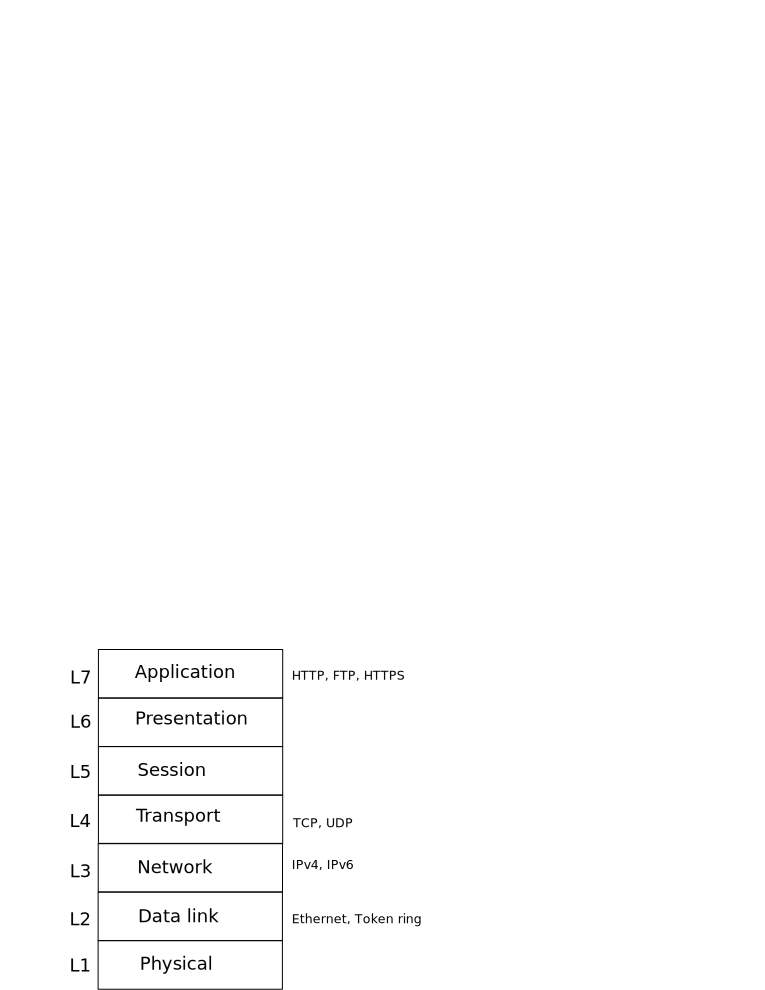
\includegraphics[scale=0.6]{chapters/pic/osi}
    \caption{Layered OSI Model; It is a conceptual model of network communication. Each layer has some task which is important for successful 
        data delivery between network services. The figure also introduces examples of typical layer protocols.}
    \label{fig:osi}
\end{figure}

As we mention in previous section, the Data Extraction is important operation of packet processing because it is typically used at each
point of network infrastructure like routers, switches, firewalls, and so on. 
Moreover, there are requests for more complex and non-trivial packet parsing. It is also the key operation for packet classification 
because results from this stage are used for searching for the best matching record.
The problem is still getting harder because the speed of network lines and parsing requirements
are still changing very dramatically. 
The main reason for this dramatic change is a growing number of communication protocols, which leads to more complicated protocol stack. 
This can be demonstrated on parsing of TCP protocol \cite{RFCTRANS} in Fig.~\ref{fig:PacketHeaderArrangement}. 
In our example, we introduce three Ethernet frames with different protocol stacks. 
This protocol arrangement leads to three various starting offsets of TCP protocol which have to be supported by the parser.
Moreover, the situation gets more complicated with Virtual Extensible LAN (VXLAN) \cite{RFCVXLAN}. 
The network virtualization technology is used to solve scalability problems in the area of cloud computing. 
It is similar to classic VLAN technology \cite{ieee2003vlan} but it encapsulates the network packets into UDP (instead of the MAC-based Ethernet frames).
The extended encapsulation leads to higher requirements on parser. 
From historical point of view, we can define two groups of parser implementation --- software and hardware based parsers.

Software based parsers are common and cheap variant of network parsers. The main component is typically the processor which 
extracts interesting data from incoming packets. 
Parser is typically a computer program which implements this functionality. This approach is also used in these days --- mainly for lower network 
speeds because the final solution is cheap and fast enough for this kind of packet processing. 
The big advantage of this solution is the flexibility of packet parser because we can react to current needs 
(parser can be easily replaced by new implementation).

\begin{figure}[t]
    \centering
    \includegraphics[scale=0.78]{chapters/pic/HeaderParsingExample}
    \caption{The example of packet header arrangement; Number represents the protocol's offset.}
    \label{fig:PacketHeaderArrangement}
\end{figure}

The second group, hardware based, is more powerful solution which is able to process much higher throughput. 
All modern high-speed network devices contains some special kind of hardware accelerated network parser. 
The disadvantage of this solution is slower development and higher cost.
There are implementation platforms like structured ASICs or FPGA circuits. 
The FPGA platform is very popular because of its flexibility, programmability and speed. 
However, hardware based parser is much harder to develop and maintain than the software version with same functionality. 
This group of network parsers still faces some challenges to solve. 
The next section describes the main approaches of hardware based packet parsers.

Braun et al. \cite{Braun02protocolwrappers} follow the idea of the layered OSI network model. 
They introduced a hardware based framework of hand-written wrappers with onion-like structure. 
For example, the parsing of the IP and UDP protocols consists of parsing of the Ethernet frame, parsing of the IP address and parsing 
of the UDP protocol. However, the detailed description of the interface is not given in the text. The FPGA implementation is able to achieve the 
throughput of 2.6\,Gbps and it is unclear how the result scales for wider data paths (i.e., higher transfer rates).

Research in this area is very intensive and researches are focused on the usage of the High-Level Synthesis (HLS). 
The HLS is typically the transformation from a higher level description to a lower level description. 
For example, Handel-C is very similar to C language. 
The HLS description is transformed to the HDL (Hardware Description Language) which is typically used for programming of FPGA circuits. 
There is a general result for the HLS approach which was given by Dedek et al. in \cite{DedekHLS}. They investigated three different realizations of
the same block. There is the comparison
of two different realizations in embedded processors (software implementation in customized 16-bit RISC and soft-core $MicroBlaze^{TM}$ processor) 
and specialized hardware based implementation with usage of Handel-C language. 
The comparison was made from different points of view: the development time, 
the estimated frequency and the occupied area. 
This work demonstrates that usage of processors gives poor results. The average throughput equals to 712\,Mbps in 
the case of custom RISC processor, 83\,Mbps for the $MicroBlaze^{TM}$ and 1454\,Mbps for the Handel-C implementation. 
The second important demonstration comes from the usage of the HLS --- the throughput and short development time can be obtained by 
usage of the higher language (Handel-C in Dedek's example).

Kobiersky et al. \cite{Kobiersky} introduce the packet header analysis and field extraction for multigigabit networks. 
The architecture for packet header processing is generated from XML protocol scheme. More than 20\,Gbps throughput can be achieved using less 
than 5000 slices of Virtex-5 FPGA.
Maximal frequency depends on the internal crossbar which doesn't scale well for wider data paths. 
However, it is the important result which shows the approach of
High-Level Synthesized network parsers in high-speed network area because it allows us to dynamically react to new network protocols. 
Unfortunately, this approach is harder to use in faster networks (like 40 and 100\,Gbps). 

A good example of HLS usage was given by Attig and Brebner \cite{AttigBrebner}. 
They introduce a PP language --- a simple high-level language for description
of packet parsing algorithms in an implementation-independent manner. 
The PP language describes the structure of packet headers and methods which define parsing rules.
The paper presents the implementation for modern FPGA which is able to accommodate high-speed network processing. 
Proposed system scales from 1 to 400\,Gbps network speeds on Virtex-7 FPGA. 
The architectural structure of the Brebner's parser is massive microcode controlled pipeline 
which consumes about 10\% of Virtex-7 resources for 1024 bits wide datapath for most common set of supported protocols 
(Ethernet, VLAN, MPLS, IPv4, IPv6, TCP and UDP). Typical disadvantage of microcode controlled solutions
is higher latency compared to pure hardware implementations. In this case, the latency varies from 292 to 548 ns.
This is inconvenient in some applications like stock exchange algorithms where the latency is crucial.  

Pu\v{s} et al. \cite{PusKekelyHfem2} proposed a novel architecture of a pipelined packet parser for FPGA based solutions, which offers 
low latency in addition to high throughput. 
These two parameters can be tuned to the needs of a particular application. Usage of such solution is very wide. The parser is 
hand-optimized thanks to the direct implementation in VHDL. 
The parser consists of analyzing blocks for variety of protocols like IPv4, IPv6, MPLS, and so on. 
Each block performs the analysis of one protocol --- it follows the main idea of layered OSI network model which was discussed in previous text. 
The communication interface of parsing blocks is generally defined and it can be used for accommodation of new protocols.
The \textit{Generic Protocol Parser Interface} (GPPI) consists of the input information which is 
needed for parsing of single protocol. The GPPI's output interface includes the parsed data and information for the next analyzer block. 
Unfortunately, the current implementation doesn't contain any HLS support despite the structure of parser is regular which makes it suitable for 
transformation from general description of parsing process. 
The parser consumes about 1.19\% of Virtex-7 FPGA resources to achieve the throughput over 100\,Gbps and 4.88\% to achieve the throughput 
over 400\,Gbps for typical set of supported protocols.

\subsection{Classification}
\label{sec:classification}
% State of the art pro klasifikaci

%Balasaheb and Kulkuhari \cite{ClasBalaAgar2013} have proposed four main groups of packet classification approaches: exhaustive search, 
%decomposition, decision tree and hierarchical-trie. 
The packet classification can be viewed as a geometrical problem of multi-dimensional discrete space searching. 
Each dimension represents one parameter which is used for the classification. 
For example, the most common classification is using five dimensions --- source and destination IP 
addresses, source and destination ports and type of transport protocol. If we combine all these parameters together, we get a 
five-dimensional search space where each point defines one packet (i.e., one combination). 
We can assign a rule to each point (or points) of given discrete space. 
The process of packet classification, from all rules containing (or we can say matching) the packet, selects one rule with the highest priority. 
The example of geometrical representation of multi-dimensinal classification is shown in Fig.~\ref{fig:GeometricRepresentationOfMultiSearchSpace}.

\begin{figure}[t]
    \centering
    \includegraphics[scale=1.2]{chapters/pic/SearchSpaceExample}
    \caption{Geometrical representation of multi-dimensional search space; Asterisk (*) represents any possible bit suffix.}
    \label{fig:GeometricRepresentationOfMultiSearchSpace}
\end{figure}

Any searching problem can be solved by searching through all available entries. We can identify two approaches --- sequential and parallel.
The first group, sequential approach, is performed by comparing the parsed headers with all the entries in the list (memory). 
The disadvantage of this approach is slow search for large set of rules because the asymptotic complexity of the 
linear probing is $\mathcal{O}(n)$. 
We can use a Ternary CAM (TCAM) engine which is used in product devices for parallel multi-dimensional packet classification. 
TCAM is a specialized memory organized in rows. Each row is composed of number of simple memory cells, where each cell can be set to three
different values 0,1 and x (\textit{don't care}). The row matches the lookup key if memory cells with 0 and 1 are equal to the corresponding bit
of lookup key. The \textit{don't care} positions are ignored, both values (0 or 1) are allowed. 
This memory is capable to match all rows in parallel. However, the complexity, cost and power consumption grows with a number of inserted rules. 
More details about this approach can be found in \cite{PusPhd}.

The decomposition based methods derive the result of classification by aggregating the individual results from searched domains, 
where the Cartesian product is typically used during the aggregation phase.
These methods offer high throughput but require
a big amount of storage space. The primary challenge is how to efficiently aggregate the results of the single field searches. 
The required storage space can be reduced by usage of pseudorules which minimize the result of the Cartesian products. It was introduced 
by Dharmapurikar et al. in \cite{DharmapurikarMSCA}.
The pseudorule is a generated rule which handles situations for packets which are not directly defined by the rule but it is needed to
obtain the correct result of the classification. However, this set of rules and pseudorules can be quite large. 
For the minimization of generated pseudorules, the Prefix Filtering Classification and Prefix Coloring Classification algorithms were 
introduced  by Pu\v{s} in \cite{PusPhd}. These approaches are able to minimize and eliminate a big amount of pseudorules
which leads to effective hardware implementation, capable to accommodate more rules and needed pseudorules. 
However, the detailed description of pseudorule concept is out of scope of this work.

Most of the classification architectures and approaches are based on direct mapping of this problem to decision trees. 
\textit{HiCuts} \cite{And99HiCuts} and \textit{HyperCuts} \cite{SingHyperCuts} are the main representatives of this approach. 
They construct a decision tree where inner tree nodes divide the space by hyperplanes 
into subspaces (e.g., it "cuts" the space into small subspaces which will be searched for the rule). 
The \textit{HyperCuts} algorithm is faster because it allows cutting on 
multiple fields per one step. However, the depth of the tree depends on a particular set because the worst case 
represents the longest path from a root to a leaf. 
The throughput strongly depends on the passed rule set (i.e., generated tree).  

Yuaxuan  et al. \cite{YaxuanFongClassification100andBeyond} introduce a tree based multi-dimensional packet classification on FPGA which is 
capable to process traffic at speed of 100\,Gbps. They used the \textit{HyperSplit} \cite{YaxuanHyperSplit} algorithm for building of optimized
\textit{k}-d classification tree. The algorithm uses heuristic for selection of most efficient splitting point on a specific protocol field. 
The paper also discusses the architecture and mapping of \textit{HyperSplit} tree to the FPGA implementation with some optimizations for 
accommodation of more classification rules. The proposed architecture is able to classify 10K rules at speed of 118\,Gbps on Virtex 6 FPGA.

Fong et al. \cite{FongWangParasplitTerabitClassification} introduce another tree based classification approach which is capable to 
hit terabit speeds. Authors introduce the \textit{ParaSplit} algorithm which uses a rule set partitioning algorithm.
The algorithm is based on range-point conversion to reduce the overall memory requirements. Authors also optimize rule partitioning 
by applying of Simulated Annealing technique. They implement the architecture for FPGA which allocates separate search engine
for each created set. Therefore, the architecture uses the native parallelism for searching of the most suitable rule in more sets in the same time.
One proposed engine is able to process 10K rules at speed of 120\,Gbps on Virtex 5 FPGA. The terabit classification is possible thanks to 
instantiation of more search engines on single chip which allows distribution of incoming traffic.

The Grid-of-Tries \cite{SrinivasanGridOfTries} is the example of hierarchical-trie approach. 
It is optimized for two dimensions but it can be extended for more dimensions. 
The algorithm uses an unibit trie \cite{EathertonUnibitTrie} for classification of one dimension. 
The result of the first trie is a pointer to the second trie, where the next dimension is being processed. 
For example, consider two dimensions ---  source and destination IP address prefixes. 
The initial trie is constructed from the source address prefixes. 
For each source address prefix node is constructed the destination address prefix trie with associated source IP address prefix. 
Therefore, the Grid-of-Tries consists of initial source address prefix trie with connected destination IP address tries. 
Search starts from the source address trie and continues with destination address trie until the desired rule is reached in a leaf. 

The most suitable algorithms, capable to hit 100\,Gbps, are based on building of decision
trees (e.g., \textit{HiCuts}, \textit{HyperCuts} or \textit{HyperSplit}) because these implementations can be effectively mapped into FPGA.
Unfortunately, the tree based algorithms have a disadvantage related to duplication of some rules which leads to higher memory consumption.
The reason of this behavior is the fact that some rules can have an intersection with two or more rule sets. Therefore, there is a need to duplicate
such rules and add them to all related sets. This disadvantage is solved by a different classification approach which is based on Cartesian
product of individual results from classification engines. The result of this operation is used for searching in a rule set (i.e., we need 
to solve if any result of Cartesian product belongs to a known rule). Advanced algorithms of this approach allow to save available memory
which has an impact on number of supported rules. However, the Cartesian product based algorithms are not suitable for usage in speeds above 10\,Gbps.
To our best knowledge, the fastest available solution for this approach was introduced by Kekely M. in \cite{KekelyP4}.
The main idea of author's architecture is based on DFCL \cite{TaylorDFCL} algorithm.
The proposed results also show that the Cartesian product based algorithms are not suitable for implementation in high-speed network devices 
capable to hit 100\,Gbps.

\subsection{General Processsing}
\label{sec:dataProcessing}
% State of the art pro obecne zpracovani

The data processing phase is typically the last stage of packet processing which is made after parsing and classification. 
It can be a general operation which is related to change of header field, stateful processing, computation of statistics, advanced 
filtering based on pattern matching, and so on. Fundamentally, we can identify two groups of general processing: 
stateless and stateful.

The first group, stateless processing, is typical for situations when the next operation (or packet processing) is not 
based on previously stored state of the flow. An example of this processing can be insertion of VLAN or MPLS tag based on result 
from the classification stage, or rewriting of IPv4 address during static NAT.

The second group, stateful processing, is more complex because next packet processing is based on the actual state which is read from internal 
memory. Therefore, this concept can implement simple or complex Finite State Machine (FSM) behavior for processing of network traffic,
where actual state and required data are stored in internal memory (state table). 
Some stateful processing engines can use the state of connection during classification phase 
(i.e., we need to connect the state memory before classification engine).
In such case, parsed headers are transferred together with read state data to following blocks (\textit{Lookup} and \textit{Update}).
The arrangement of state memory depends on needs of implemented application. The main concept is shown in Fig.~\ref{fig:StatefulProcessing}. 
Incoming headers and corresponding state are passed to the \textit{Lookup} block where the engine looks for the most suitable action. 
After that, the block passes required data (headers, state and selected action) to the \textit{Update} block where the selected action is executed. 
The action can be related to data change, update of the state data, and so on. 
The last step, write back of new state data, is optional and it depends on implemented application.

\begin{figure}[ht]
    \centering
    \includegraphics[scale=0.75]{chapters/pic/StatefulProcessing}
    \caption{General scheme of stateful processing.}
    \label{fig:StatefulProcessing}
\end{figure}

Application area of stateful processing is wide and we cannot introduce all possibilities.  
However, we select a frequent application to provide the basic overview.
Traffic measurement (also called as per-flow statistics collection) is a typical example of this approach.
It is required in many network application like security, accounting, real-time traffic analysis, and so on. 
We provide more details about this kind of processing in following text.

\subsubsection*{Traffic Measurement}
Fundamentally, the traffic measurement involves counting number of packets (update operation) which meet some criteria. Moreover, the update 
criteria can be much more complex. For example, we can use statistical methods for detection of anomalous traffic. The traffic is measured 
in terms of \textit{flows}. The flow refers to a set of packets which have the same \textit{n}-tuple in their header field. 
The \textit{n}-tuple typically consists of five members: \textit{\{sip,dip,spt,dpt,prt\}} where, \textit{sip} and \textit{dip} stands for 
source and destination IP, \textit{spt} and 
\textit{dpt} stands for source and destination port. Finally, the \textit{prt} stands for the type of L4 transport protocol such as TCP or UDP. 

NetFlow is considered to be a traditional measurement scheme. 
It is based on storage of per-flow records on high-density media.
This stored data is processed later to find the answer on the query. 
This technology requires three components --- \textit{NetFlow exporter}, \textit{NetFlow collector} and \textit{NetFlow statistics storage}. 
\textit{NetFlow statistics} are sampled from network devices such as routers, switches or network probes, to network collector. 

\begin{figure}[ht]
	\centering
	\includegraphics[scale=0.3]{chapters/pic/NetFlow}
	\caption{Brief NetFlow architecture.}
	\label{fig:netflowArchitecture}
\end{figure}

All aggregated statistics are stored by the \textit{NetFlow collector} to the \textit{Per-Flow statistics storage}. 
The most modern collectors and exporters support insertion of information from application layer (L7) which makes user queries much more complex. 
Discussed architecture is shown in Fig.~\ref{fig:netflowArchitecture}. 
Measured statistics are processed by usage of queries which are created by the operator. 
The answer of the query is computed on a \textit{NetFlow collector }
(for example – the number of received bytes of flow with specific IP address and source TCP port). 
The main disadvantage can be a higher latency of detection.

\begin{figure}[b]
    \centering
    \includegraphics[scale=0.57]{chapters/pic/sdm_arch}
    \caption{Brief SDM Architecture.}
    \label{fig:sdmArch}
\end{figure}

The \textit{Software Defined Monitoring} \cite{KekelyPusKorenekSDM} is the example of advanced flow based monitoring with hardware accelerated extension.
The main idea of this approach is to offload the uninteresting flows into the hardware accelerated analyzer while the 
interesting flows are sent to the software for deeper and more complex analysis. It eliminates the lack of scalability for faster interfaces. 
Moreover, it connects the world of high-speed networking and HLS. 
This connection is based on our research which was introduced in \cite{PusBenacekSDMUpdate}.
We demonstrated the ability of FPGAs and HLS tools available today to extend the 
functionality of the hardware by new instructions (new types of aggregation functions).
While the typical use of HLS is the synthesis of digital signal processing algorithms,
we employ a C/C++ to VHDL synthesizer to implement the instructions of the application specific processor.
We implemented the processor infrastructure in VHDL and prepare it for a wide variety of instructions.
Finally, we evaluate the approach by implementing five different instructions (two of them being NetFlow like, three non-NetFlow) in 
High-Level Language (HLL) to assess the versatility of the HLS for the task of processor instruction description.
The SDM consists of two main parts (firmware and software) connected together via PCI Express bus. 
Both parts are tightly coupled together to allow a precise control of the hardware processing on the per-flow basis.
The software part of SDM consists of the controller and monitoring applications. 
Advanced monitoring tasks, such as analysis of application protocols, are performed in the monitoring applications.
The management of the hardware (removing and insertion of the processing rules) is performed in the controller.
The SDM Processor hardware is controlled by instructions stored in rules.
The instruction tells the hardware what action must be performed for each input packet.
The hardware passes the data to the software in the form of packet metadata (extracted information from the packet header) or aggregated 
flow records (NetFlow for example).
Whole received packet can be also sent to the software for deeper analysis. Graphical representation of the SDM concept is shown 
in Fig.~\ref{fig:sdmArch}.


\section{Languages and Abstractions of Network Devices}
% V teto kapitole budeme popisovat jazyky, ktere se daji pouzit pro definici sitovych zarizeni v dostatecne obecne mire. Budou
% nasledovat kapitoly s blizsim popisem a pripadnyma ukazkama

The following text introduces modern languages and abstractions of packet processing devices, together with code examples.

\subsection{OpenFlow}
OpenFlow \cite{openflow}, as the most popular embodiment of the ideas of Software-Defined Networking \cite{SDNSpec},
provides a way to fill the lookup tables of switches at runtime.
The OpenFlow specification defines exactly which protocols are supported by switches. 
At the same time, it is not possible to change the set of supported protocols or actions --- switches are fixed 
(or at least they appear so to the OpenFlow controller).

\begin{figure}[b]
    \centering
    \includegraphics[scale=0.75]{chapters/pic/OpenFlowConcept}
    \caption{Architecture of packet processing device with OpenFlow support.}
    \label{fig:openflow_processing}
\end{figure}

Architecture of packet processing device with OpenFlow support is given in Fig.~\ref{fig:openflow_processing}. 
Whole concept contains several components:
\begin{itemize}
   \item \textbf{OpenFlow Controller} is a centralized component which controls more OpenFlow switches.
   It is used for configuration of OpenFlow switches at runtime. That is, it defines mapping between protocol fields
   and used actions. The action can be related to protocol field change, packet drop, forwarding of processed packet to next table, and so on. 
   Therefore, the OpenFlow Controller defines a behavior of forwarding plane by filling the tables with rules.
   The example of OpenFlow Controller is Ryu \cite{RyuController} which is available under open source license.
   \item \textbf{OpenFlow communication protocol} gives the access to the forwarding plane of SDN switch. It also defines a set of supported
   protocols, actions and tables. These sets typically depend on version of OpenFlow.  
   The latest specification is from April 2015 (OpenFlow version 1.5.1 \cite{OpenFlowSpec}).
   \item \textbf{OpenFlow Switch} is the realization of forwarding plane (software or hardware based implementation). 
   All capabilities are defined by supported version of OpenFlow protocol. OpenFlow Switch typically consists of several tables.
   As we noticed in previous text, the behavior of the forwarding plane is defined by rules which are inserted to lookup tables at runtime.
   The most important is the \textit{Flow table} which is used for implementation of match and action functionality. 
   That is, it uses protocol fields of processed packet for identification of the most suitable action which is executed in the same table. 
   OpenFlow switch typically contains more \textit{Flow Tables} which are used for implementation of more complex match and action behavior.
   The \textit{Group table} supports sets of actions for flooding as well as more complex forwarding semantics 
   (e.g., multipath, fast reroute, and link aggregation).
   Finally, the \textit{Meter table} consists of per-flow meter entries, which enable OpenFlow to implement various QoS operations.
\end{itemize}

The packet, entering OpenFlow switch, is processed by the parser which identifies available protocol fields. These fields are used as a key for 
searching of most suitable action in first \textit{Flow table}. 
The searched action is executed if the \textit{Flow table} founds matching record. 
In the case of tables miss, the \textit{miss-action} handler is activated. Typically, the non-matching packet is sent to
SDN Controller for further processing which can lead to insertion of new rule (i.e., the logic of network application is implemented
in controller and it decides about the future of given flow).

The detailed description of SDN and OpenFlow is out of scope of this work. 
However, we provide basic pros and cons of this approach. The main advantage is the direct programmability of forwarding plane
from \textit{OpenFlow Controller}. Simply said, the controller defines the logic of network forwarding. This logic (or some part of it) is 
translated to the form of rules which are uploaded to tables in \textit{SDN Switch}. The second advantage is connected with central management
of the SDN network which is beneficial for maintaining of global view on the network.
As we noticed before, the main disadvantage is connected with limited set of supported protocols and actions which cannot be extended
(i.e., any new functionality has to be emulated in software). This behavior is inconvenient in high-speed networks because network
device has to process big amount of packets in a short time. This need leads to an extensible forwarding plane which bypasses
the emulation of new functionality in software.

\subsection{Gorilla}
% Info v paperu: Compiling hight throughput network processors (Gorilla Compiling hight throughput network processors (Gorilla))
% paper opsahuje nejake info, vytahnout ten jazyk, dostupnou vykonnost
%
% Poznamky:
% - gorilla pouziva templaty, ktere zapoji do pipeliny nebo multivlaknove architektury, vsechny moduly ale musi byt implementovany predem a my je jenom vyuzivame. To je sice
% fajn ale oproti P4 to neumoznuje tu flexibilitu. Uzivatel je tak zavisly na HDL koderovi, protoze mu musi poskytnout modul pro procesovani protokolu.
% - takze zrovna parser muze byt popsat v P4 a bude mit stejnou funkcionalitu  (P4 je silnejsi) 
% - dosahli 100G, ale porad to neni dostatecne flexibilni v porovnani s P4
% - maji neco jako deparser, ale rikaji tomu Post-processing
% - matchovani delaji ve specialnich akceleratorech
% - delali designy pro 10, 50 a 100G v ruznych konfiguracich
Lavasani, Denninson and Chiou introduced the Gorilla methodology in \cite{GorillaFPGA2012}. This methodology is used for compilation of high throughput 
network processors from abstract description. 
The main goal is to abstract network engineers from underlying hardware. 
The Gorilla methodology defines canonical and general architecture for implementation of variety of network applications. 
The Gorilla's compiler accepts an abstract description which is translated to a Verilog source code. 
The translation process uses highly parameterized templates which are created by a skilled HDL designer. 
All modules can be connected in pipelined or multithreaded manner. 
The multithreaded hardware supports more "threads", where each thread does a specific unit of work.

The proposed approach allows to find a trade-off between consumed resources and reached throughput with retained generality. 
Network engineer can describe the packet processing in a language similar to C notation. The following example is taken from \cite{GorillaFPGA2012}:

\begin{Verbatim}[fontsize=\small]
IPv4_check() {
    status = IPv4_header_integrity_check(Header);
    if (status == CHKSUM_OK)
        Next_step = IPv4_lookup;
    else
        Next_step = Exception;
}

IPv4_lookup() {
    Da_class = lookupx.search(Header.IPv4_dstaddr);
    Sa_class = lookupy.search(Header.IPv4_srcaddr);
    if (Da_class == NOT_FOUND)
        Next_step = Exception;
    else if(Sa_class == NOT_FOUND)
        Next_step = Exception;
    else
        Next_step = IPv4_modify;
}

IPv4_modify() {
    if((IP_update_fields(Header) == ZERO_TTL))
        Next_step = Exception;
    else {
        Dport = Da_class.dport;
    Next_step = Emit;
    }
}
\end{Verbatim}

Authors of the proposed methodology provide performance results for the FPGA implementation. 
The Xilinx Virtex-5 TX240T FPGA (used on NetFPGA-10G board) was
used for implementation of the IPv4 lookup. The Xilinx Virtex-6 HX380T FPGA was used for implementation of 50\,Gbps multi-protocol stack
(IPv4, IPv6 and MPLS).
Finally, the Xilinx Virtex-7 VHX870T was used for implementation of 100\,Gbps multi-protocol engine. 
All cores were able to hit the target throughput on 64 byte Ethernet packets at frequency of 100\,MHz.
These results make the Gorilla very suitable for implementation of high-speed network processors.

However, the proposed methodology uses templates of processing engines and packet parsers which makes the Gorilla somewhat static. 
The example of this static behavior is the inability to extend the set of supported protocols and packet parsers during development of network application 
(i.e., Gorilla supports the limited set of protocols which are supported by the HDL template library). 
The Gorilla methodology is intended to be used in FPGA only.

\subsection{SDNet}
% Zkusit dohledat nejake ukazky, informace.
% 
% Pokud mozno potvrdit:
% Vyhoda naseho reseni je to, ze oproti SDNetu mame zdrojovy kod dostupny, v jejich pripade je uzavreny, aby uzivatel nemohl
% delat zadne zmeny. To neumoznuje jemne ladeni kodu + neumoznuje implementovat zadne vylepseni.

The SDNet \cite{XilinxSDNet} is a commercial solution from Xilinx. 
The PX language is used for abstract description of packet processing devices. 
We provide the example of Ethernet parsing that has been taken from \cite{XilinxSDNet}:

\begin{Verbatim}[fontsize=\small]
class OF_parser::ParsingEngine (9000,4) {
    // Tuple class for extracted data
    class Flow :: Tuple(inout) {
        struct flow_s { // OpenFlow 12-tuple
        port:3,
        dmac:48,smac:48,type:16, // Eth
        vid:12,pcp:3, // VLAN
        sa:32,da:32,proto:8,tos:6, // IP
        sp:16,dp:16 // TCP
    }
}

Flow fields;
// Section class for Ethernet header
class ETH :: Section {
    struct {dmac:48, smac:48, type:16}
    method update = {
    fields.dmac = dmac,
    fields.smac = smac,
    fields.type = type
    }
method move_to_section =
    if (type == 0x8100) VLAN
    else if (type == 0x0800) IP
    else done(1);
    method increment_offset = size();
}

// VLAN, IP, TCP classes follow ...
// Similar style to ETH class
}
\end{Verbatim}

The complete parser declaration contains a declaration of the header format, together with methods that 
define selection of next processed protocol (i.e., it defines the type of next used protocol) and computation of the next starting offset. 
The rule searching engines supports three classes of algorithms: Content addressable memory (CAM), Longest-prefix match
and ternary CAM.
Users of SDNet can define a composed design from parsers and user defined processing engines. Such definition requires specification
of an interconnection pattern between used modules. 
The following example of MPLS LSR system with Secret Sauce user engine has been taken from 
\cite{XilinxSDNet} (interconnection is defined in \textit{connect} method):

\begin{Verbatim}[fontsize=\small]
class MPLS_LSR::System {
    // Input and output interfaces
    Packet_input instream;
    Packet_output outstream;

    // Sub-engines
    MPLS_Classifier classifier;
    Secret_Sauce relay;
    MPLS_Editor editor;

    // Interconnections
    method connect = {
    classifier.packetin = instream,
    relay.in = classifier.packetout,
    editor.packetin = relay.out,
    editor.fields = classifier.fields,
    editor.op = classifier.op,
    outstream = editor.packetout
    }
}

// ...
class Secret_Sauce :: UserEngine {
    Packet_input in;
    Packet_output out;
}
\end{Verbatim}

The SDNet proposes a flexible solution capable to scale line rates from 1\,Gbps to 100\,Gbps. The PX language is a modern and powerful concept for 
description of high-speed packet processing engines. Xilinx also introduced a translator from P4 (se later) to PX language in \cite{XilinxP4toPX}. 
However, the Xilinx SDNet is closed system which doesn't allow implementation of novel hardware approaches 
(i.e., all changes have to be made by Xilinx). 
This is complicated for network researchers because they have to wait for implementation of novel algorithms and hardware architectures in SDNet. 
Therefore, there is a need for open and customizable solution which is suitable for translation from high-level description to HDL language.

\subsection{OpenState}
OpenState \cite{OpenStateSpec,BianchiOpenState,OpenStateGithub} is a research effort focused on development of a stateful data plane and API for SDN. 
Authors of this approach proposed an extension to current OpenFlow abstraction that uses state machines implemented inside switches to reduce 
the need to rely on remote controllers. It also introduces usage of \textit{eXtended Finite State Machines} 
(XFSM; more in \cite{BianchiWirelessMacProcessor,BianchiMaclets}). 
This extension allows implementation of complex stateful behavior like port knocking, DDoS detection/mitigation, and so on. 

\begin{figure}[ht]
    \centering
    \includegraphics[width=0.95\textwidth]{chapters/pic/OpenStateConcept}
    \caption{OpenState concept (taken from \protect\cite{OpenStateSpec}).}
    \label{fig:OpenStateConcept}
\end{figure}

Basic OpenState concept is shown in Fig.~\ref{fig:OpenStateConcept}. As defined by OpenFlow, a packet is processing through the 
pipeline of tables where each table provides the match and action functionality. 
Firstly, the entering packet is processed by \textit{Key extractor} which produces a key
based on configuration of \textit{lookup-scope}. The key is used for identification of state in \textit{State table}. 
The matched state data is transferred together with packet headers to \textit{Flow table}. This table is extended with matching of state which 
can be understood as a virtual protocol field (i.e., it isn't the part of a protocol but it is used for matching). 
Outputs from \textit{Flow table} are following --- (1)~packet headers with suitable action
and (2)~updated state information. The update is written to the \textit{State table} based on configuration of \textit{update-scope}. 
The pros and cons are summarized in following lists:
\begin{itemize}
    \item \textbf{Pros:}
        \begin{itemize}
            \item Based on existing proven standard (OpenFlow).
            \item Powerful stateful processing.
        \end{itemize}
    \item \textbf{Cons:}
        \begin{itemize}
            \item Feedback loop complicates implementation. It may require synchronization among CPU threads, pipeline stalls in FPGA/ASIC.
            \item Non-extensible protocol and action support.
        \end{itemize}
\end{itemize}

\subsection{P4}
\label{sec:p4Language}
% Napsat jazyku P4, ze je to nova vec, definuje nejake zakladni aspekty
% 1) Popis protokolu
% 2) Popis parseru
% 3) Popis match+actio tabulky
% 4) Popis akci
% 5) Popis kontrolniho programu
% 
% Je to otevreny standard, ktery se vytvari, proto podrobneji popiseme jednotlive aspekty jazyka
P4 (Programming Protocol-independent Packet Processors) \cite{p4,p4web} is an open source, high-level and platform-agnostic language.
It represents a recent contribution to the broader idea of Software-Defined Networking (SDN) and its ecosystem. 
Its main purpose is to provide a way to define packet processing functionality of network devices, paying attention to reconfigurability in the field,
protocol independence and target platform independence. Using relatively simple syntax, P4 allows to define five aspects of packet processing:
\begin{itemize}
\item \textbf{Header Formats} describe protocol headers recognized by the device.
\item \textbf{Packet Parser} describes the (conceptual) state machine used to traverse packet headers from start to end, extracting field values 
as it goes.
\item \textbf{Table Specification} defines how the extracted header fields are matched in possibly multiple lookup tables 
(e.g., exact match, prefix match and range search).
\item \textbf{Action Specification} defines compound actions that may be executed for packets.
\item \textbf{Control Program} puts all the above together, defining the control flow mainly among the tables.
\end{itemize}

All proposed aspects can be mapped to three operations of packet processing. The Header Formats and Packer Parser describes the structure 
of incoming data and relations between protocols. 
We can map these two aspects to the Packet Parsing. The Table Specification generally describes the process of classification. 
In general, the classification uses the extracted data for searching of most suitable processing rule. 
The Action Specification is used for definition of general processing action.
The Control Program specifies the sequence of classification and action stages. 
Therefore, we can divide the classification and action blocks to more stages which allows us to implement more complex behavior. 
We also demonstrate the usability and flexibility of this language, compared to existing SDN ecosystem, in \cite{2016cesnet-p4,2016root-p4}.
The following text provides examples of syntax and further details of P4 language.

\subsubsection*{Header Definition}
% Tady se popise vice podrobneji jak se definuje popis hlavicky. Ze je nejaka staticka, dynamicka .. atd.

Header Definition is very similar to declaration of structure in C language. 
The P4 language uses a simple syntax in the form of \textit{name} : \textit{width}. 
Header Definition for the Ethernet header looks like this:

\begin{Verbatim}[fontsize=\small]
header ethernet {
   fields {
      dstAddr   : 48; // width in bits
      srcAddr   : 48;
      ethertype : 16;
   }
}
\end{Verbatim}

The description simply lists fields of the packet header and their width in bits. 
The example above shows a protocol with static header structure, where the header length is the sum of lengths of all fields. 
This can't be done for protocols with variable header length. 
The P4 language solves this situation by the header length definition in the form of an expression which uses fields from the protocol header 
declaration to compute the header length. Header Definition with variable length may looks like this:
\begin{Verbatim}[fontsize=\small]
header_type ipv6_ext_t {
    fields {
        nextHdr     : 8;
        totalLen    : 8;
        frag        : 12;
        padding     : 3;
        fragLast    : 1;
    }

    length     : (totalLen + 1) * 8;
    max_length : 1024; // Bytes
}
\end{Verbatim}

\subsubsection*{Parser Definition}
\label{sec:p4ParserDefinition}
% Tady se podrobneji popise definice parseru s nejakyma ukazkama, s maskou atd.
Parser Definition is used for the description of relations between protocol headers
That is, it defines one state of FSM which describes the parsing process in terms of transitions between protocols. 
Parser Definition may looks like this:

\begin{Verbatim}[fontsize=\small]
header ethernet eth;
parser parse_ethernet {
   extract(eth);
   switch(eth.ethertype) {
      case 0x8100: vlan;
      case 0x9100: vlan;
      case 0x0800: ipv4;
      case 0xA100 mask 0xF100 : myProto;
      default : ingress;
   }
}
\end{Verbatim}

The provided example uses \textit{switch} and \textit{extract} statements. 
The \textit{extract} statement instructs the parser to examine input packets and to look for data defined in the header. 
Parsed data is then used in the \textit{switch} statement to determine the next state (protocol) to process. There are also situations when
we don't want to use the whole value from the protocol field. The P4 language solves this with the \textit{mask} 
statement which is used in the \textit{case} statement together with mask value. In our example, the \textit{mask} statement instructs 
the P4 parser to take the \textit{ethertype} field, perform logical $and$ operation between the value and mask. 
Finally, the result is compared to \textit{0xA100} value. 
The \textit{switch} statement can contain not only references to next parsers but it can also contain references to Control Flows. 
Such references instruct the P4 program to stop parsing and continue with processing of extracted data.
The entrance point of each P4 program is the parser with \textit{start} name, for example:
\begin{Verbatim}[fontsize=\small]
 parser start {
    return parse_ethernet;
}
\end{Verbatim}

\subsubsection*{Match+Action Table Definition}
\label{subsubsec:matchActionTableDefinition}
% Tady se podorobneji popise match+action tabulka, co to je, struktura a tak
The Match+Action Table is used for mapping of extracted header fields to most suitable action. The Match+Action Table consists of:
\begin{enumerate}
    \item \textbf{Extracted header fields} - these fields are used for identification of record in Match+Action Table. 
    Each referenced field contains the declaration of algorithm which is used for matching. The list of supported matches is following: 
    \textit{exact}, the \textit{Longest Prefix Match} (LPM), \textit{range}, \textit{valid} and \textit{ternary} match. 
    The \textit{exact} match is working with value without any masking. The LPM is the most common matching algorithm 
    in IP protocol which is based on looking for the longest binary prefix in passed data. 
    The \textit{ternary} match is more general than LPM because 
    it allows us to work with three bit values - logical \textit{1}, logical \textit{0} and \textit{don't care}. 
    Therefore, LPM is a special case of \textit{ternary} match. 
    The \textit{range} match is used for matching on range of values. Finally, the \textit{valid} match checks the presence of used
    protocol header in processed packet.
    \item \textbf{List of supported actions} - this declaration contains the list of supported actions which can be used from the particular table.
\end{enumerate}

The example of Match+Action Table definition in P4 language can be following:
\begin{Verbatim}[fontsize=\small]
    table filter {
        reads {
            ipv4.srcAddr    : lpm;
            tcp.dstPort     : exact;
        }

        actions {
            PushVlan;
            Permit;
            NoOp;
        }   
    }
\end{Verbatim}

The proposed example uses two protocols for matching (all used fields are listed in the \textit{reads} statement). 
The fist one is the source address of IPv4 protocol which uses the LPM algorithm for matching. 
The second one, TCP port, uses the \textit{exact} match.
Finally, the list of supported actions is defined in the \textit{actions} statement. 
Actions can be filled with some parameters. These parameters are stored within the record in the Match+Action Table. 
More details about declaration of actions are situated in following text.

\subsubsection*{Action Definition}
% Tady se popise podrobneji definice akci, ze jsou nejake defaultni a ze si muze uzivatel definovat sve vlastni
The P4 language defines the list of primitives actions (see the P4 language specification in \cite{p4languagespec}). 
These primitive actions can be combined to more complex user actions. 
Each user defined action can call other user defined or primitive actions. 
The following example is taken from \cite{p4languagespec}:
\begin{Verbatim}[fontsize=\small]
    action add_mTag(up1, up2, down1, down2, egr_spec) {
        add_header(mTag);
        // Copy VLAN ethertype to mTag
        copy_field(mTag.ethertype, vlan.ethertype);
        // Set the VLAN's ethertype to signal mTag
        copy_field(vlan.ethertype,0xaaaa);
        set_field(mTag.up1, up1);
        set_field(mTag.up2, up2);
        set_field(mTag.down1, down1);
        set_field(mTag.down2, down2);
        // Set the destination egress port as well
        set_field(metadata.egress_spec, egr_spec);
    }
\end{Verbatim}

All action are performed in sequential manner. The action can be imagined as a function in C language (the syntax is similar). 
The action can accept some parameters. As was mentioned in previous text, these parameters are stored within record in the Match+Action Table 
and we can configure these parameters during runtime (i.e., configuration of the P4 device from software tool).
In our example, the mTag header (user defined) is inserted after the VLAN header. 
To do that, we need to copy the ethertype value from the VLAN header to mTag, and setup the VLAN ethertype to 0xaaaa
(we want to signalize the presence of the mTag protocol). Finally, we setup the rest of the mTag fields and value of output port.

\subsubsection*{Control Flow Definition}
% Tady se popise podrobneji specifikace kontorlniho programu, ze jsou tam nejak ify, ze se volaji pomoci apply
% ty tabulky a tak
We defined headers, parser, tables and user defined actions. Finally, we need to define the ordering of Match+Action Tables in program.
This behavior is defined in the P4's Control Flow. We start the description with simple example (the code is taken from \cite{p4languagespec}):
\begin{Verbatim}[fontsize=\small]
    control ingress {
        // Verify the mTag state and port 
        apply(source_check);
        // If no error from source_check, continue
        if(!defined(metadata.ingress_error)) {
            // Attempt to switch to end host
            apply(local_switching);
            if(!defined(metadata.egress_spec)) {
                // Not a known local host
                apply(mTag_table);
            }
            // Check for unknown egress state or bad retagging with mTag
            apply(egress_check);
        }
    }
\end{Verbatim}

Match+Action Tables are executed using the \textit{apply} statement. The control block typically consists of \textit{apply} and \textit{if-else} 
statements. Used tables can be selected regarding to hit/miss in previous table, selected action, and so on.
Therefore, we can implement a quite complex behavior of packet processing. 
The full description of all available functionality can be found in \cite{p4languagespec}.

\section{Summary}
% Tady se napise nejake zhodnoceni, ze jsme uvedli aktualni veci a ze jsme predstavili P4 jazyk. Nicmene, bylo uvedeno 
% pouze par paperu na generovani celeho sitoveho zarizeni. 
%
% Dale napsat, ze ten P4 jazyk je otevreny a tak bude nejvhodnejsi jako vstupni bod pro nase mapovani na efektivni implementaci
% jednotlivych bloku v FPGA implementaci. 
We introduced and described three network operation groups --- parsing, classification and general processing. 
The latest and most modern solutions for each operation were described. 
Finally, we introduced high-level solutions for description of packet processing functionality --- Gorilla, SDNet and P4.
The Gorilla is one of the first approaches for description of high-speed network devices but the solution is somewhat static in term
of extensibility (new protocols and actions). 
The SDNet is the latest and most modern approach capable to scale from 1\,Gbps to 400\,Gbps. However, this technology is 
closed which makes it quite hard to extend it with newest FPGA based hardware solutions from network area. 
The P4 language is a complex language for specification of modern packet processing devices which is developed under open-source license. 
The specification also introduced the P4 language as a platform independent solution which makes it usable not only in FPGAs. 
We also demonstrate the usability, platform independence and flexibility of this language, compared to existing SDN ecosystem, in 
\cite{2016cesnet-p4,2016root-p4}. Therefore, we will focus on P4 in following text.
